%iffalse
\let\negmedspace\undefined
\let\negthickspace\undefined
\documentclass[journal,12pt,onecolumn]{IEEEtran}
\usepackage{cite}
\usepackage{amsmath,amssymb,amsfonts,amsthm}
\usepackage{algorithmic}
\usepackage{graphicx}
\usepackage{textcomp}
\usepackage{xcolor}
\usepackage{txfonts}
\usepackage{listings}
\usepackage{enumitem}
\usepackage{mathtools}
\usepackage{gensymb}
\usepackage{comment}
\usepackage[breaklinks=true]{hyperref}
\usepackage{tkz-euclide} 
\usepackage{listings}
\usepackage{gvv}                                        
%\def\inputGnumericTable{}                                 
\usepackage[latin1]{inputenc}     
\usepackage{xparse}
\usepackage{color}                                            
\usepackage{array}                                            
\usepackage{longtable}                                       
\usepackage{calc}                                             
\usepackage{multirow}
\usepackage{multicol}
\usepackage{hhline}                                           
\usepackage{ifthen}                                           
\usepackage{lscape}
\usepackage{tabularx}
\usepackage{array}
\usepackage{float}
\newtheorem{theorem}{Theorem}[section]
\newtheorem{problem}{Problem}
\newtheorem{proposition}{Proposition}[section]
\newtheorem{lemma}{Lemma}[section]
\newtheorem{corollary}[theorem]{Corollary}
\newtheorem{example}{Example}[section]
\newtheorem{definition}[problem]{Definition}
\newcommand{\BEQA}{\begin{eqnarray}}
\newcommand{\EEQA}{\end{eqnarray}}
\usepackage{float}
\theoremstyle{remark}
\usepackage{ circuitikz }


\title{GATE-EC-2022}
\author{EE25BTECH11002 - Achat Parth Kalpesh }
\date{}

\begin{document}

\maketitle

\section*{Q.1 - Q.5  Carry ONE mark each. }

\begin{enumerate}
    \item Mr. X speaks \rule{2cm}{0.4pt} Japanese \rule{2cm}{0.4pt} Chinese.

    \hfill{(GATE EC 2022)}
    \begin{enumerate}
        \begin{multicols}{2}
            \item neither / or
            \item either / nor
            \item neither / nor
            \item also / but
        \end{multicols}
    \end{enumerate}

    \item A sum of money is to be distributed among P, Q, R, and S in the proportion $5:2:4:3$, respectively.
    If R gets Rs. 1000 more than S, what is the share of Q \brak{\text{in Rs. }}?

    \hfill{(GATE EC 2022)}
    \begin{enumerate}
    \begin{multicols}{4}
        \item 500
        \item 1000
        \item 1500
        \item 2000
    \end{multicols}
    \end{enumerate}

    \item A trapezium has vertices marked as P, Q, R and S \brak{\text{in that order anticlockwise}}. The side PQ is parallel to side SR.
    Further, it is given that, PQ = 11 cm, QR = 4 cm, RS = 6 cm and SP = 3 cm.
    What is the shortest distance between PQ and SR \brak{\text{in cm}}?

    \hfill{(GATE EC 2022)}
    \begin{enumerate}
        \begin{multicols}{4}
        \item 1.80
        \item 2.40
        \item 4.20
        \item 5.76
    \end{multicols}
    \end{enumerate}

    \item The figure shows\figref{fig:m1} a grid formed by a collection of unit squares. The unshaded unit square in the grid represents a hole.
    \begin{figure}[H]
        \centering
        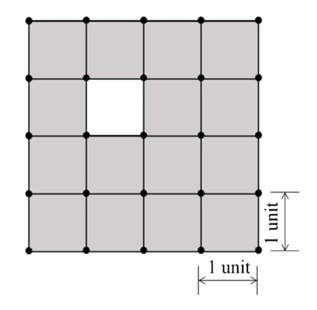
\includegraphics[width=0.4\columnwidth]{figs/m1.jpg}
        \caption*{}
        \label{fig:m1}
    \end{figure}
    What is the maximum number of squares without a "hole in the interior" that can be formed within the $4 \times 4$ grid using the unit squares as building blocks?

    \hfill{(GATE EC 2022)}
    \begin{enumerate}
        \begin{multicols}{4}
        \item 15
        \item 20
        \item 21
        \item 26
     \end{multicols}   
    \end{enumerate}

    \item An art gallery engages a security guard to ensure that the items displayed are protected. The diagram below\figref{fig:m2} represents the plan of the gallery where the boundary walls are opaque. The location the security guard posted is identified such that all the inner space \brak{\text{shaded region in the plan}} of the gallery is within the line of sight of the security guard.
    \begin{figure}[H]
        \centering
        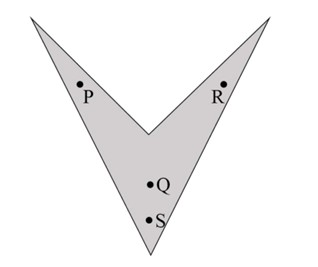
\includegraphics[width=0.3\columnwidth]{figs/m2.jpg}
        \caption*{}
        \label{fig:m2}
    \end{figure}
    If the security guard does not move around the posted location and has a $360\degree$ view, which one of the following correctly represents the set of ALL possible locations among the locations P, Q, R and S, where the security guard can be posted to watch over the entire inner space of the gallery.

    \hfill{(GATE EC 2022)}
    \begin{enumerate}
        \begin{multicols}{4}
        \item P and Q
        \item Q
        \item Q and S
        \item R and S
    \end{multicols}
    \end{enumerate}

    \textbf{Q. 6 - Q. 10  Carry TWO marks each.}

    \item Mosquitoes pose a threat to human health. Controlling mosquitoes using chemicals may have undesired consequences. In Florida, authorities have used genetically modified mosquitoes to control the overall mosquito population. It remains to be seen if this novel approach has unforeseen consequences.
    Which one of the following is the correct logical inference based on the information in the above passage?

    \hfill{(GATE EC 2022)}
    \begin{enumerate}
        \item Using chemicals to kill mosquitoes is better than using genetically modified mosquitoes because genetic engineering is dangerous
        \item Using genetically modified mosquitoes is better than using chemicals to kill mosquitoes because they do not have any side effects
        \item Both using genetically modified mosquitoes and chemicals have undesired consequences and can be dangerous
        \item Using chemicals to kill mosquitoes may have undesired consequences but it is not clear if using genetically modified mosquitoes has any negative consequence
    \end{enumerate}

    \item Consider the following inequalities.
    \begin{enumerate}
        \item $2x - 1 > 7$
        \item $2x - 9 < 1$
    \end{enumerate}
    Which one of the following expressions below satisfies the above two inequalities?

    \hfill{(GATE EC 2022)}
    \begin{enumerate}
        \begin{multicols}{4}
        \item $x \leq -4$
        \item $-4 < x \leq 4$
        \item $4 < x < 5$
        \item $x \geq 5$
        \end{multicols}
    \end{enumerate}

    \item Four points $P\brak{0, 1}$, $Q\brak{0, -3}$, $R\brak{-2, -1}$, and $S\brak{2, -1}$ represent the vertices of a quadrilateral.
    What is the area enclosed by the quadrilateral?

    \hfill{(GATE EC 2022)}
    \begin{enumerate}
        \begin{multicols}{4}
        \item 4
        \item $4\sqrt{2}$
        \item 8
        \item $8\sqrt{2}$
        \end{multicols}
    \end{enumerate}

    \item In a class of five students P, Q, R, S and T, only one student is known to have copied in the exam. The disciplinary committee has investigated the situation and recorded the statements from the students as given below.
    
    \textbf{Statement of P:} R has copied in the exam.
    
    \textbf{Statement of Q:} S has copied in the exam.
    
    \textbf{Statement of R:} P did not copy in the exam.
    
    \textbf{Statement of S:} Only one of us is telling the truth.
    
    \textbf{Statement of T:} R is telling the truth.
    
    The investigating team had authentic information that S never lies.
    Based on the information given above, the person who has copied in the exam is

    \hfill{(GATE EC 2022)}
    \begin{enumerate}
        \begin{multicols}{4}
        \item R
        \item P
        \item Q
        \item T
        \end{multicols}
    \end{enumerate}

\textbf{Q.11 - Q.35 Carry ONE mark Each}

    \item Consider the following square\figref{fig:m3} with the four corners and the center marked as P, Q, R, S and T respectively.
    \begin{figure}[H]
        \centering
        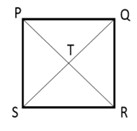
\includegraphics[width=0.25\columnwidth]{figs/m3.jpg}
        \caption*{}
        \label{fig:m3}
    \end{figure}
    Let X, Y and Z represent the following operations:
    
    X: rotation of the square by 180 degree with respect to the S-Q axis.
    
    Y: rotation of the square by 180 degree with respect to the P-R axis.
    
    Z: rotation of the square by 90 degree clockwise with respect to the axis perpendicular, going into the screen and passing through the point T.
    
    Consider the following three distinct sequences of operation \brak{\text{which are applied in the left to right order}}.
    \begin{enumerate}
        \item XYZZ
        \item XY
        \item ZZZZ
    \end{enumerate}
    Which one of the following statements is correct as per the information provided above?

    \hfill{(GATE EC 2022)}
    \begin{enumerate}
        \item The sequence of operations \brak{1} and \brak{2} are equivalent
        \item The sequence of operations \brak{1} and \brak{3} are equivalent
        \item The sequence of operations \brak{2} and \brak{3} are equivalent
        \item The sequence of operations \brak{1}, \brak{2} and \brak{3} are equivalent
    \end{enumerate}

    \item Consider the two-dimensional vector field $\vec{F}\brak{x, y} = x\hat{i} + y\hat{j}$, where $\hat{i}$ and $\hat{j}$ denote the unit vectors along the x-axis and the y-axis, respectively. A contour $C$ in the x-y plane, as shown in the figure,\figref{fig:m4} is composed of two horizontal lines connected at the two ends by two semicircular arcs of unit radius. The contour is traversed in the counter-clockwise sense. The value of the closed path integral
    \begin{align*}
        \oint_C \vec{F}\brak{x, y} \cdot \brak{dx\hat{i} + dy\hat{j}}
    \end{align*}
    is \rule{2cm}{0.4pt}.
    \begin{figure}[H]
        \centering
        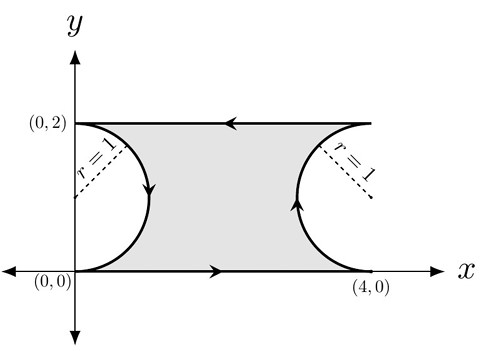
\includegraphics[width=0.5\columnwidth]{figs/m4.jpg}
        \caption*{}
        \label{fig:m4}
    \end{figure}

    \hfill{(GATE EC 2022)}
    \begin{enumerate}
    \begin{multicols}{4}
        \item 0
        \item 1
        \item $8 + 2\pi$
        \item -1
    \end{multicols}
    \end{enumerate}

    \item Consider a system of linear equations $Ax = b$, where
    \begin{align*}
        A = \myvec{1 & -\sqrt{2} \\ -1 & \sqrt{2}},  b = \myvec{1 \\ 3}
    \end{align*}
    This system of equations admits \rule{2cm}{0.4pt}.

    \hfill{(GATE EC 2022)}
    \begin{enumerate}
    \begin{multicols}{2}
        \item a unique solution for x
        \item infinitely many solutions for x
        \item no solutions for x
        \item exactly two solutions for x
        \end{multicols}
    \end{enumerate}

    \item The current $I$ in the circuit shown\figref{fig:m5} is \rule{2cm}{0.4pt}.
    \begin{figure}[H]
        \centering
        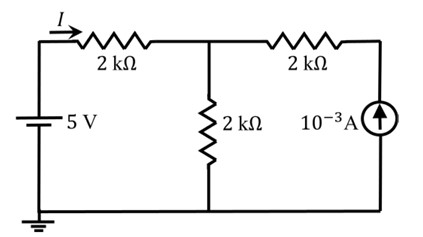
\includegraphics[width=0.5\columnwidth]{figs/m5.jpg}
        \caption*{}
        \label{fig:m5}
    \end{figure}

    \hfill{(GATE EC 2022)}
    \begin{enumerate}
    \begin{multicols}{4}
        \item $1.25 \times 10^{-3}$ A
        \item $0.75 \times 10^{-3}$ A
        \item $-0.5 \times 10^{-3}$ A
        \item $1.16 \times 10^{-3}$ A
        \end{multicols}
    \end{enumerate}

    \item Consider the circuit shown in the figure.\figref{fig:m6} The current $I$ flowing through the $10 \ohm$ resistor is \rule{2cm}{0.4pt}.
    \begin{figure}[H]
        \centering
        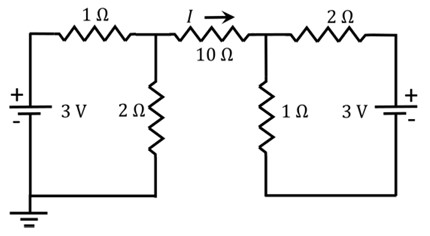
\includegraphics[width=0.5\columnwidth]{figs/m6.jpg}
        \caption*{}
        \label{fig:m6}
    \end{figure}

    \hfill{(GATE EC 2022)}
    \begin{enumerate}
    \begin{multicols}{4}
        \item 1 A
        \item 0 A
        \item 0.1 A
        \item -0.1 A
        \end{multicols}
    \end{enumerate}

    \item The Fourier transform $X\brak{j\omega}$ of the signal
    \begin{align*}
        x\brak{t} = \frac{t}{\brak{1+t^2}^2}
    \end{align*}
    is \rule{2cm}{0.4pt}.

    \hfill{(GATE EC 2022)}
    \begin{enumerate}
    \begin{multicols}{4}
        \item $\frac{\pi}{2j} \omega e^{-\abs{\omega}}$
        \item $\frac{\pi}{2} \omega e^{-\abs{\omega}}$
        \item $\frac{\pi}{2j} e^{-\abs{\omega}}$
        \item $\frac{\pi}{2} e^{-\abs{\omega}}$
        \end{multicols}
    \end{enumerate}

    \item Consider a long rectangular bar of direct bandgap p-type semiconductor. The equilibrium hole density is $10^{17} \text{ cm}^{-3}$ and the intrinsic carrier concentration is $10^{10} \text{ cm}^{-3}$. Electron and hole diffusion lengths are $2 \mu\text{m}$ and $1 \mu\text{m}$, respectively.
    The left side of the bar \brak{x=0} is uniformly illuminated with a laser having photon energy greater than the bandgap of the semiconductor. Excess electron-hole pairs are generated ONLY at $x = 0$ because of the laser. The steady state electron density at $x = 0$ is $10^{14} \text{ cm}^{-3}$ due to laser illumination. Under these conditions and ignoring electric field, the closest approximation \brak{\text{among the given options}} of the steady state electron density at $x = 2 \mu\text{m}$, is \rule{2cm}{0.4pt}.

    \hfill{(GATE EC 2022)}
    \begin{enumerate}
    \begin{multicols}{2}
        \item $0.37 \times 10^{14} \text{ cm}^{-3}$
        \item $0.63 \times 10^{13} \text{ cm}^{-3}$
        \item $3.7 \times 10^{14} \text{ cm}^{-3}$
        \item $10^3 \text{ cm}^{-3}$
        \end{multicols}
    \end{enumerate}

    \item In a non-degenerate bulk semiconductor with electron density $n = 10^{16} \text{ cm}^{-3}$, the value of $E_C - E_{Fn} = 200 \text{ meV}$, where $E_C$ and $E_{Fn}$ denote the bottom of the conduction band energy and electron Fermi level energy, respectively. Assume thermal voltage as 26 meV and the intrinsic carrier concentration is $10^{10} \text{ cm}^{-3}$. For $n = 0.5 \times 10^{16} \text{ cm}^{-3}$, the closest approximation of the value of $\brak{E_C - E_{Fn}}$, among the given options, is \rule{2cm}{0.4pt}.

    \hfill{(GATE EC 2022)}
    \begin{enumerate}
        \begin{multicols}{4}
            \item 226 meV
            \item 174 meV
            \item 218 meV
            \item 182 meV
        \end{multicols}
    \end{enumerate}
    
    \item Consider the CMOS circuit shown in the figure\figref{fig:m7} \brak{\text{substrates are connected to their respective sources}}. The gate width \brak{W} to gate length \brak{L} ratios \brak{\frac{W}{L}} of the transistors are as shown. Both the transistors have the same gate oxide capacitance per unit area. For the pMOSFET, the threshold voltage is -1 V and the mobility of holes is $40 \ \frac{\text{cm}^2}{\text{V.s}}$. For the nMOSFET, the threshold voltage is 1 V and the mobility of electrons is $300 \ \frac{\text{cm}^2}{\text{V.s}}$. The steady state output voltage $V_O$ is \rule{2cm}{0.4pt}.
    \begin{figure}[H]
        \centering
        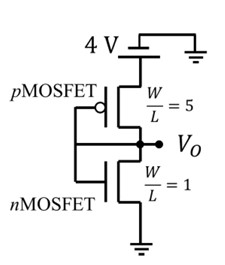
\includegraphics[width=0.3\columnwidth]{figs/m7.jpg}
        \caption*{}
        \label{fig:m7}
    \end{figure}
    
    \hfill{(GATE EC 2022)}
    \begin{enumerate}
    \begin{multicols}{2}
        \item equal to 0 V
        \item more than 2 V
        \item less than 2 V
        \item equal to 2 V
        \end{multicols}
    \end{enumerate}

    \item Consider the 2-bit multiplexer \brak{MUX} shown in the figure.\figref{fig:m8} For OUTPUT to be the XOR of C and D, the values for $A_0, A_1, A_2$, and $A_3$ are \rule{2cm}{0.4pt}.
    \begin{figure}[H]
        \centering
        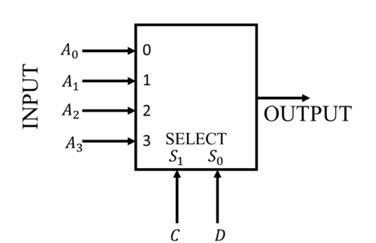
\includegraphics[width=0.5\columnwidth]{figs/m8.jpg}
        \caption*{}
        \label{fig:m8}
    \end{figure}

    \hfill{(GATE EC 2022)}
    \begin{enumerate}
    \begin{multicols}{2}
        \item $A_0 = 0, A_1 = 0, A_2 = 1, A_3 = 1$
        \item $A_0 = 1, A_1 = 0, A_2 = 1, A_3 = 0$
        \item $A_0 = 0, A_1 = 1, A_2 = 1, A_3 = 0$
        \item $A_0 = 1, A_1 = 1, A_2 = 0, A_3 = 0$
        \end{multicols}
    \end{enumerate}

    \item The ideal long channel nMOSFET and pMOSFET devices shown\figref{fig:m9} in the circuits have threshold voltages of 1 V and -1 V, respectively. The MOSFET substrates are connected to their respective sources. Ignore leakage currents and assume that the capacitors are initially discharged. For the applied voltages as shown, the steady state voltages are \rule{2cm}{0.4pt}.
    \begin{figure}[H]
        \centering
        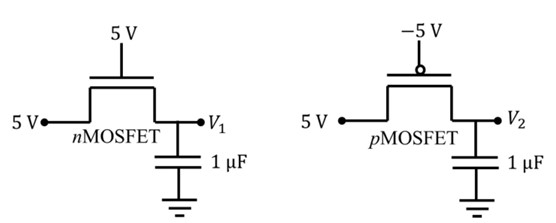
\includegraphics[width=0.5\columnwidth]{figs/m9.jpg}
        \caption*{}
        \label{fig:m9}
    \end{figure}

    \hfill{(GATE EC 2022)}
    \begin{enumerate}
        \begin{multicols}{2}
            \item $V_1 = 5 \text{ V},  V_2 = 5 \text{ V}$
            \item $V_1 = 5 \text{ V},  V_2 = 4 \text{ V}$
            \item $V_1 = 4 \text{ V},  V_2 = 5 \text{ V}$
            \item $V_1 = 4 \text{ V},  V_2 = -5 \text{ V}$
        \end{multicols}
    \end{enumerate}

    \item Consider a closed-loop control system with unity negative feedback and $KG\brak{s}$ in the forward path, where the gain $K=2$. The complete Nyquist plot of the transfer function $G\brak{s}$ is shown in the figure.\figref{fig:m10} Note that the Nyquist contour has been chosen to have the clockwise sense. Assume $G\brak{s}$ has no poles on the closed right-half of the complex plane. The number of poles of the closed-loop transfer function in the closed right-half of the complex plane is \rule{2cm}{0.4pt}.
    \begin{figure}[H]
        \centering
        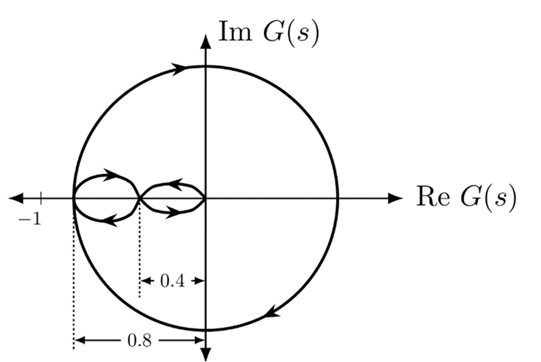
\includegraphics[width=0.5\columnwidth]{figs/m10.jpg}
        \caption*{}
        \label{fig:m10}
    \end{figure}

    \hfill{(GATE EC 2022)}
    \begin{enumerate}
    \begin{multicols}{4}
        \item 0
        \item 1
        \item 2
        \item 3
        \end{multicols}
    \end{enumerate}

    \item The root-locus plot of a closed-loop system with unity negative feedback and transfer function $KG\brak{s}$ in the forward path is shown in the figure.\figref{fig:m11} Note that K is varied from 0 to $\infty$.
    Select the transfer function $G\brak{s}$ that results in the root-locus plot of the closed-loop system as shown in the figure.
    \begin{figure}[H]
        \centering
        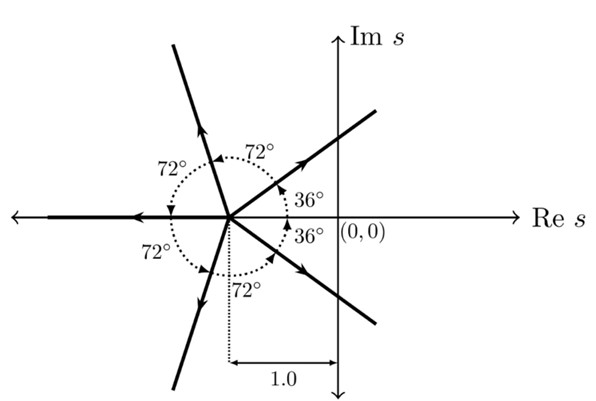
\includegraphics[width=0.5\columnwidth]{figs/m11.jpg}
        \caption*{}
        \label{fig:m11}
    \end{figure}

    \hfill{(GATE EC 2022)}
    \begin{enumerate}
    \begin{multicols}{2}
        \item $G\brak{s} = \frac{1}{\brak{s+1}^5}$
        \item $G\brak{s} = \frac{1}{s^5+1}$
        \item $G\brak{s} = \frac{s-1}{\brak{s+1}^6}$
        \item $G\brak{s} = \frac{s+1}{s^6+1}$
        \end{multicols}
    \end{enumerate}

    \item The frequency response $H\brak{f}$ of a linear time-invariant system has magnitude as shown in the figure.\figref{fig:m12}
    \begin{figure}[H]
        \centering
        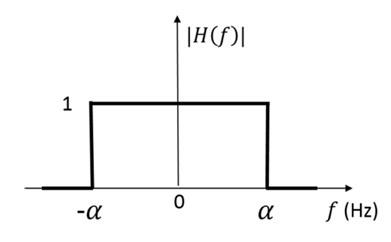
\includegraphics[width=0.4\columnwidth]{figs/m12.jpg}
        \caption*{}
        \label{fig:m12}
    \end{figure}
    \textbf{Statement I:} The system is necessarily a pure delay system for inputs which are bandlimited to $-\alpha \leq f \leq \alpha$.
    
    \textbf{Statement II:} For any wide-sense stationary input process with power spectral density $S_X\brak{f}$, the output power spectral density $S_Y\brak{f}$ obeys $S_Y\brak{f} = S_X\brak{f}$ for $-\alpha \le f \le \alpha$.
    
    Which one of the following combinations is true?

    \hfill{(GATE EC 2022)}
    \begin{enumerate}
        \item Statement I is correct, Statement II is correct
        \item Statement I is correct, Statement II is incorrect
        \item Statement I is incorrect, Statement II is correct
        \item Statement I is incorrect, Statement II is incorrect
    \end{enumerate}

    \item In a circuit, there is a series connection of an ideal resistor and an ideal capacitor. The conduction current \brak{\text{in Amperes}} through the resistor is $2\sin\brak{t+\pi/2}$. The displacement current \brak{\text{in Amperes}} through the capacitor is \rule{2cm}{0.4pt}.
    
    \hfill{(GATE EC 2022)}
    \begin{enumerate}
    \begin{multicols}{4}
        \item $2\sin\brak{t}$
        \item $2\sin\brak{t+\pi}$
        \item $2\sin\brak{t+\pi/2}$
        \item 0
        \end{multicols}
    \end{enumerate}

    \item Consider the following partial differential equation \brak{PDE}
    \begin{align*}
        a \frac{\partial^2 f\brak{x,y}}{\partial x^2} + b \frac{\partial^2 f\brak{x,y}}{\partial y^2} = f\brak{x,y},
    \end{align*}
    where $a$ and $b$ are distinct positive real numbers. Select the combination\brak{s} of values of the real parameters $\xi$ and $\eta$ such that $f\brak{x,y} = e^{\brak{\xi x + \eta y}}$ is a solution of the given PDE.

    \hfill{(GATE EC 2022)}
    \begin{enumerate}
        \item $\xi = \frac{1}{\sqrt{2a}},  \eta = \frac{1}{\sqrt{2b}}$
        \item $\xi = \frac{1}{\sqrt{a}},  \eta = 0$
        \item $\xi = 0, \eta = 0$
        \item $\xi = \frac{1}{\sqrt{a}}, \eta = \frac{1}{\sqrt{b}}$
    \end{enumerate}

    \item An ideal OPAMP circuit with a sinusoidal input is shown in the figure.\figref{fig:m13} The 3 dB frequency is the frequency at which the magnitude of the voltage gain decreases by 3 dB from the maximum value. Which of the options is/are correct?
    \begin{figure}[H]
        \centering
        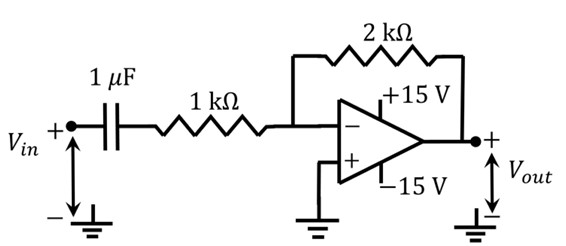
\includegraphics[width=0.5\columnwidth]{figs/m13.jpg}
        \caption*{}
        \label{fig:m13}
    \end{figure}

    \hfill{(GATE EC 2022)}
    \begin{enumerate}
    \begin{multicols}{2}
        \item The circuit is a low pass filter.
        \item The circuit is a high pass filter.
        \item The 3 dB frequency is 1000 rad/s.
        \item The 3 dB frequency is $\frac{1000}{3}$ rad/s.
        \end{multicols}
    \end{enumerate}

    \item Select the Boolean function\brak{s} equivalent to $x+yz$, where $x, y,$ and $z$ are Boolean variables, and + denotes logical OR operation.

    \hfill{(GATE EC 2022)}
    \begin{enumerate}
    \begin{multicols}{2}
        \item $x + z + xy$
        \item $\brak{x+y}\brak{x+z}$
        \item $x + xy + yz$
        \item $x + xz + xy$
        \end{multicols}
    \end{enumerate}

    \item Select the correct statement\brak{s} regarding CMOS implementation of NOT gates.

    \hfill{(GATE EC 2022)}
    \begin{enumerate}
        \item Noise Margin High \brak{NM_H} is always equal to the Noise Margin Low \brak{NM_L}, irrespective of the sizing of transistors.
        \item Dynamic power consumption during switching is zero.
        \item For a logical high input under steady state, the nMOSFET is in the linear regime of operation.
        \item Mobility of electrons never influences the switching speed of the NOT gate.
    \end{enumerate}

    \item Let $H\brak{X}$ denote the entropy of a discrete random variable $X$ taking $K$ possible distinct real values. Which of the following statements is/are necessarily true?

    \hfill{(GATE EC 2022)}
    \begin{enumerate}
    \begin{multicols}{2}
        \item $H\brak{X} \leq \log_2 K$ bits
        \item $H\brak{X} \leq H\brak{2X}$
        \item $H\brak{X} \leq H\brak{X^2}$
        \item $H\brak{X} \leq H\brak{2^X}$
        \end{multicols}
    \end{enumerate}

    \item Consider the following wave equation,
    \begin{align*}
        \frac{\partial^2 f\brak{x,t}}{\partial t^2} = 10000 \frac{\partial^2 f\brak{x,t}}{\partial x^2}
    \end{align*}
    Which of the given options is/are solution\brak{s} to the given wave equation?

    \hfill{(GATE EC 2022)}
    \begin{enumerate}
        \item $f\brak{x,t} = e^{-\brak{x-100t}^2} + e^{-\brak{x+100t}^2}$
        \item $f\brak{x,t} = e^{-\brak{x-100t}} + 0.5 e^{-\brak{x+1000t}}$
        \item $f\brak{x,t} = e^{-\brak{x-100t}} + \sin\brak{x+100t}$
        \item $f\brak{x,t} = e^{j100\pi\brak{-100x+t}} + e^{j100\pi\brak{100x+t}}$
    \end{enumerate}

    \item The bar graph\figref{fig:m14} shows the frequency of the number of wickets taken in a match by a bowler in her career. For example, in 17 of her matches, the bowler has taken 5 wickets each. The median number of wickets taken by the bowler in a match is \rule{2cm}{0.4pt} \brak{\text{rounded off to one decimal place}}.
    \begin{figure}[H]
        \centering
        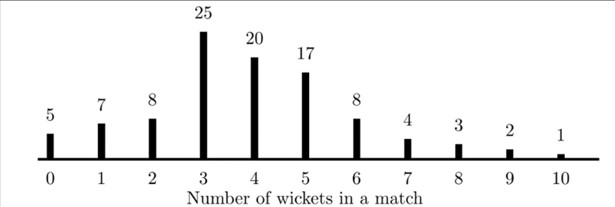
\includegraphics[width=0.5\columnwidth]{figs/m14.jpg}
        \caption*{}
        \label{fig:m14}
    \end{figure}

    \hfill{(GATE EC 2022)}

    \item A simple closed path C \figref{fig:m15} in the complex plane is shown in the figure. If
    \begin{align*}
        \oint_C \frac{2^z}{z^2-1} dz = -i\pi A,
    \end{align*}
    where $i = \sqrt{-1}$, then the value of A is \rule{2cm}{0.4pt} \brak{\text{rounded off to two decimal places}}.
    \begin{figure}[H]
        \centering
        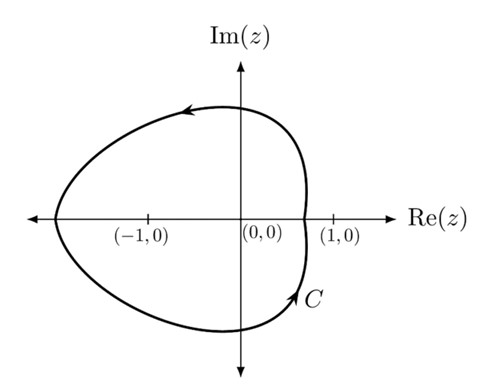
\includegraphics[width=0.5\columnwidth]{figs/m15.jpg}
        \caption*{}
        \label{fig:m15}
    \end{figure}

    \hfill{(GATE EC 2022)}

    \item Let $x_1\brak{t} = e^{-t}u\brak{t}$ and $x_2\brak{t} = u\brak{t} - u\brak{t-2}$, where $u\brak{\cdot}$ denotes the unit step function.
    If $y\brak{t}$ denotes the convolution of $x_1\brak{t}$ and $x_2\brak{t}$, then $\lim_{t\to\infty} y\brak{t} =$ \rule{2cm}{0.4pt} \brak{\text{rounded off to one decimal place}}.
    
    \hfill{(GATE EC 2022)}

    \item An ideal MOS capacitor \brak{\text{p-type semiconductor}} is shown in the figure.\figref{fig:m16}  The MOS capacitor is under strong inversion with $V_G = 2$ V. The corresponding inversion charge density \brak{Q_{IN}} is $2.2  \mu\text{C/cm}^2$. Assume oxide capacitance per unit area as $C_{ox} = 1.7  \mu\text{F/cm}^2$. For $V_G = 4$ V, the value of $Q_{IN}$ is \rule{2cm}{0.4pt} $\mu\text{C/cm}^2$ \brak{\text{rounded off to one decimal place}}.
    \begin{figure}[H]
        \centering
        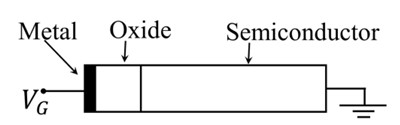
\includegraphics[width=0.5\columnwidth]{figs/m16.jpg}
        \caption*{}
        \label{fig:m16}
    \end{figure}
    
    \hfill{(GATE EC 2022)}

    \item A symbol stream contains alternate QPSK and 16-QAM symbols. If symbols from this stream are transmitted at the rate of 1 mega-symbols per second, the raw \brak{\text{uncoded}} data rate is \rule{2cm}{0.4pt} mega-bits per second \brak{\text{rounded off to one decimal place}}.
    
    \hfill{(GATE EC 2022)}

\textbf{Q. 36 - Q. 65  Carry TWO marks each.}

    \item The function $f\brak{x} = 8\log_e x - x^2 + 3$ attains its minimum over the interval $\sbrak{1, e}$ at $x = $ \rule{2cm}{0.4pt}. \brak{\text{Here } \log_e x \text{ is the natural logarithm of } x}.
    
    \hfill{(GATE EC 2022)}
    \begin{enumerate}
    \begin{multicols}{4}
        \item 2
        \item 1
        \item $e$
        \item $\frac{1+e}{2}$
        \end{multicols}
    \end{enumerate}

    \item Let $\alpha, \beta$ be two non-zero real numbers and $v_1, v_2$ be two non-zero real vectors of size $3 \times 1$. Suppose that $v_1$ and $v_2$ satisfy $v_1^T v_2 = 0$, $v_1^T v_1 = 1$, and $v_2^T v_2 = 1$. Let $A$ be the $3 \times 3$ matrix given by:
    \begin{align}
     A = \alpha v_1 v_1^T + \beta v_2 v_2^T 
     \end{align}
    The eigenvalues of A are \rule{2cm}{0.4pt}.
    
    \hfill{(GATE EC 2022)}
    \begin{enumerate}
    \begin{multicols}{4}
        \item $0, \alpha, \beta$
        \item $0, \alpha+\beta, \alpha-\beta$
        \item $0, \frac{\alpha+\beta}{2}, \sqrt{\alpha\beta}$
        \item $0, 0, \sqrt{\alpha^2+\beta^2}$
        \end{multicols}
    \end{enumerate}

    \item For the circuit shown,\figref{fig:m17}  the locus of the impedance $Z\brak{j\omega}$ is plotted as $\omega$ increases from zero to infinity. The values of $R_1$ and $R_2$ are:
    \begin{figure}[H]
        \centering
        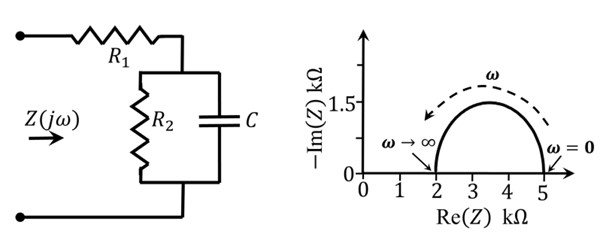
\includegraphics[width=0.5\columnwidth]{figs/m17.jpg}
        \caption*{}
        \label{fig:m17}
    \end{figure}
    
    \hfill{(GATE EC 2022)}
    \begin{enumerate}
    \begin{multicols}{2}
        \item $R_1 = 2$ k$\ohm$, $R_2 = 3$ k$\ohm$
        \item $R_1 = 5$ k$\ohm$, $R_2 = 2$ k$\ohm$
        \item $R_1 = 5$ k$\ohm$, $R_2 = 2.5$ k$\ohm$
        \item $R_1 = 2$ k$\ohm$, $R_2 = 5$ k$\ohm$
        \end{multicols}
    \end{enumerate}

    \item Consider the circuit shown in the figure\figref{fig:m18}  with input $V\brak{t}$ in volts. The sinusoidal steady state current $I\brak{t}$ flowing through the circuit is shown graphically \brak{\text{where } t \text{ is in seconds}}. The circuit element Z can be \rule{2cm}{0.4pt}.
    \begin{figure}[H]
        \centering
        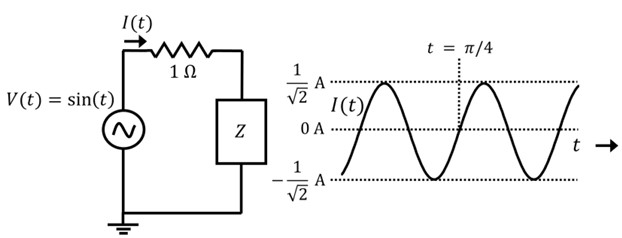
\includegraphics[width=0.5\columnwidth]{figs/m18.jpg}
        \caption*{}
        \label{fig:m18}
    \end{figure}
    
    \hfill{(GATE EC 2022)}
    \begin{enumerate}
    \begin{multicols}{2}
        \item a capacitor of 1 F
        \item an inductor of 1 H
        \item a capacitor of $\sqrt{3}$ F
        \item an inductor of $\sqrt{3}$ H
        \end{multicols}
    \end{enumerate}

    \item Consider an ideal long channel nMOSFET \brak{\text{enhancement-mode}} with gate length 10 $\mu$m and width 100 $\mu$m. The product of electron mobility \brak{\mu_n} and oxide capacitance per unit area \brak{\text{$C_{ox}$}} is $\mu_n$ $C_{ox}$ = 1 mA/V$^2$. The threshold voltage of the transistor is 1 V. For a gate-to-source voltage $V_{GS}$ = $\sbrak{2 - \sin\brak{2t}}$ V and drain-to-source voltage $V_{DS}$ = 1 V \brak{\text{substrate connected to the source}}, the maximum value of the drain-to-source current is \rule{2cm}{0.4pt}.
    
    \hfill{(GATE EC 2022)}
    \begin{enumerate}
    \begin{multicols}{4}
        \item 40 mA
        \item 20 mA
        \item 15 mA
        \item 5 mA
        \end{multicols}
    \end{enumerate}
    
    \item For the following circuit\figref{fig:m19}  with an ideal OPAMP, the difference between the maximum and the minimum values of the capacitor voltage \brak{V_C} is \rule{2cm}{0.4pt}.
    \begin{figure}[H]
        \centering
        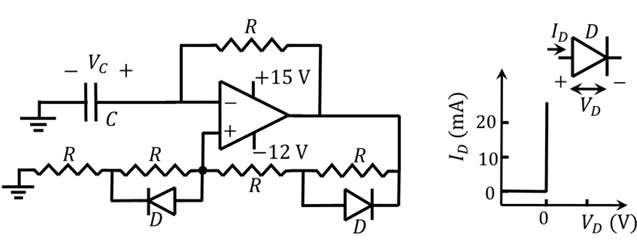
\includegraphics[width=0.9\columnwidth]{figs/m19.jpg}
        \caption*{}
        \label{fig:m19}
    \end{figure}
    
    \hfill{(GATE EC 2022)}
    \begin{enumerate}
    \begin{multicols}{4}
        \item 15 V
        \item 27 V
        \item 13 V
        \item 14 V
        \end{multicols}
    \end{enumerate}

    \item A circuit with an ideal OPAMP is shown.\figref{fig:m20}  The Bode plot for the magnitude \brak{\text{in dB}} of the gain transfer function \brak{A_V\brak{j\omega} = V_{out}\brak{j\omega}/V_{in}\brak{j\omega}} of the circuit is also provided \brak{\text{here, } \omega \text{ is the angular frequency in rad/s}}. The values of R and C are \rule{2cm}{0.4pt}.
    \begin{figure}[H]
        \centering
        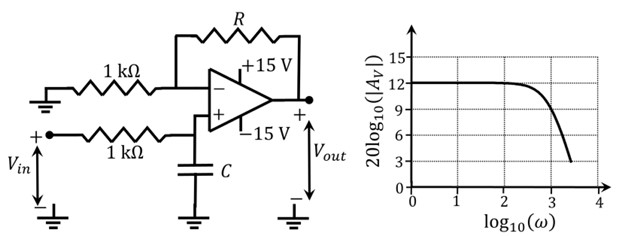
\includegraphics[width=\columnwidth]{figs/m20.jpg}
        \caption*{}
        \label{fig:m20}
    \end{figure}
    
    \hfill{(GATE EC 2022)}
    \begin{enumerate}
    \begin{multicols}{2}
        \item R = 3 k$\ohm$, C = 1 $\mu$F
        \item R = 1 k$\ohm$, C = 3 $\mu$F
        \item R = 4 k$\ohm$, C = 1 $\mu$F
        \item R = 3 k$\ohm$, C = 2 $\mu$F
        \end{multicols}
    \end{enumerate}

    \item For the circuit shown,\figref{fig:m21} the clock frequency is $f_0$ and the duty cycle is 25\%. For the signal at the Q output of the Flip-Flop, \rule{2cm}{0.4pt}.
    \begin{figure}[H]
        \centering
        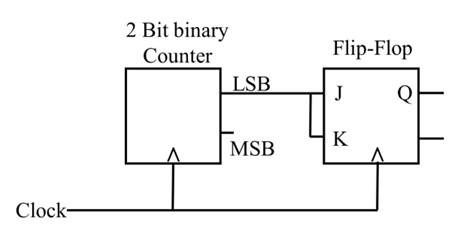
\includegraphics[width=0.5\columnwidth]{figs/m21.jpg}
        \caption*{}
        \label{fig:m21}
    \end{figure}
    
    \hfill{(GATE EC 2022)}
    \begin{enumerate}
    \begin{multicols}{2}
        \item frequency is $f_0/4$ and duty cycle is 50\%
        \item frequency is $f_0/4$ and duty cycle is 25\%
        \item frequency is $f_0/2$ and duty cycle is 50\%
        \item frequency is $f_0$ and duty cycle is 25\%
        \end{multicols}
    \end{enumerate}

    \item Consider an even polynomial $p\brak{s}$ given by
    \begin{align*}
    p\brak{s} = s^4 + 5s^2 + 4 + K,
    \end{align*} 
    where K is an unknown real parameter. The complete range of K for which $p\brak{s}$ has all its roots on the imaginary axis is \rule{2cm}{0.4pt}.
    
    \hfill{(GATE EC 2022)}
    \begin{enumerate}
    \begin{multicols}{4}
        \item $-4 \leq K \leq \frac{9}{4}$
        \item $-3 \leq K \leq \frac{9}{2}$
        \item $-6 \leq K \leq \frac{5}{4}$
        \item $-5 \leq K \leq 0$
        \end{multicols}
    \end{enumerate}

    \item Consider the following series:
    \begin{align*}
    \sum_{n=1}^{\infty} \frac{n^d}{c^n} 
    \end{align*}
    For which of the following combinations of $c, d$ values does this series converge?
    
    \hfill{(GATE EC 2022)}
    \begin{enumerate}
    \begin{multicols}{4}
        \item $c=1, d=-1$
        \item $c=2, d=1$
        \item $c=0.5, d=-10$
        \item $c=1, d=-2$
        \end{multicols}
    \end{enumerate}

    \item The outputs of four systems \brak{S_1, S_2, S_3 and S_4} corresponding to the input signal $\sin\brak{t}$, for all time $t$, are shown in the figure.\figref{fig:m22} Based on the given information, which of the four systems is/are definitely NOT LTI \brak{\text{linear and time-invariant}}?
    \begin{figure}[H]
        \centering
        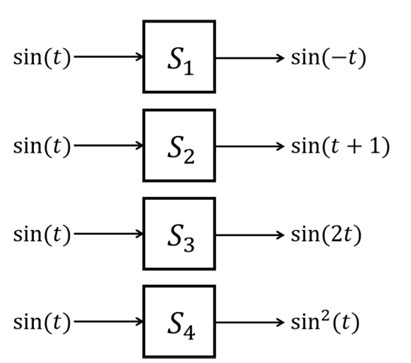
\includegraphics[width=0.5\columnwidth]{figs/m22.jpg}
        \caption*{}
        \label{fig:m22}
    \end{figure}
    
    \hfill{(GATE EC 2022)}
    \begin{enumerate}
        \begin{multicols}{4}
            \item $S_1$
            \item $S_2$
            \item $S_3$
            \item $S_4$
        \end{multicols}
    \end{enumerate}

    \item Select the CORRECT statement\brak{s} regarding semiconductor devices.
    
    \hfill{(GATE EC 2022)}
    \begin{enumerate}
        \item Electrons and holes are of equal density in an intrinsic semiconductor at equilibrium.
        \item Collector region is generally more heavily doped than Base region in a BJT.
        \item Total current is spatially constant in a two terminal electronic device in dark under steady state condition.
        \item Mobility of electrons always increases with temperature in Silicon beyond 300 K.
    \end{enumerate}

    \item A state transition diagram with states A, B, and C, and transition probabilities $p_1, p_2, \dots, p_7$ is shown in the figure\figref{fig:m23}  \brak{\text{e.g., } p_1 \text{ denotes the probability of transition from state A to B}}. For this state diagram, select the statement\brak{s} which is/are universally true.
    \begin{figure}[H]
        \centering
        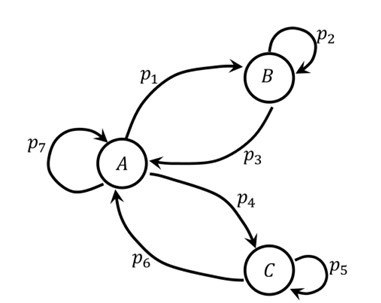
\includegraphics[width=0.5\columnwidth]{figs/m23.jpg}
        \caption*{}
        \label{fig:m23}
    \end{figure}
    
    \hfill{(GATE EC 2022)}
    \begin{enumerate}
    \begin{multicols}{2}
        \item $p_2 + p_3 = p_5 + p_6$
        \item $p_1 + p_3 = p_4 + p_6$
        \item $p_1 + p_4 + p_7 = 1$
        \item $p_2 + p_5 + p_7 = 1$
        \end{multicols}
    \end{enumerate}

    \item Consider a Boolean gate \brak{D} where the output Y is related to the 
    inputs A and B as, $Y = A + B$, where $+$ denotes logical OR operation. The
    Boolean inputs '0' and '1' are also available separately. Using instances of 
    only D gates and inputs '0' and '1', \rule{2cm}{0.4pt} \brak{\text{select the correct option\brak{s}}}.
    
    \hfill{(GATE EC 2022)}
    \begin{enumerate}
    \begin{multicols}{2}
        \item NAND logic can be implemented
        \item OR logic cannot be implemented
        \item NOR logic can be implemented
        \item AND logic cannot be implemented
        \end{multicols}
    \end{enumerate}

    \item Two linear time-invariant systems with transfer functions
    \begin{align}
    G_1\brak{s} = \frac{10}{s^2+s+1}  \text{ and } G_2\brak{s} = \frac{10}{s^2+s\sqrt{10}+10} 
    \end{align}
    have unit step responses $y_1\brak{t}$ and $y_2\brak{t}$, respectively. Which of the following statements is/are true?
    
    \hfill{(GATE EC 2022)}
    \begin{enumerate}
        \item $y_1\brak{t}$ and $y_2\brak{t}$ have the same percentage peak overshoot.
        \item $y_1\brak{t}$ and $y_2\brak{t}$ have the same steady-state value.
        \item $y_1\brak{t}$ and $y_2\brak{t}$ have the same damped frequency of oscillation.
        \item $y_1\brak{t}$ and $y_2\brak{t}$ have the same 2\% settling time.
    \end{enumerate}
    
    \item Consider an FM broadcast that employs the pre-emphasis filter with frequency response
    \begin{align*}
    H_{pe}\brak{\omega} = 1 + \frac{j\omega}{\omega_0},
    \end{align*}
    where $\omega_0 = 10^4$ rad/sec. For the network shown in the figure\figref{fig:m24}  to act as a corresponding de-emphasis filter, the appropriate pair\brak{s} of \brak{R, C} values is/are \rule{2cm}{0.4pt}.
    \begin{figure}[H]
        \centering
        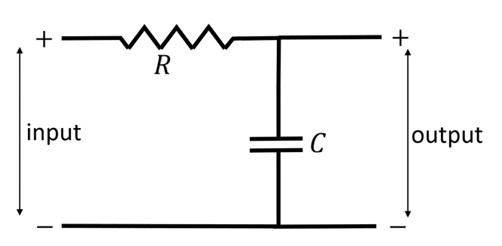
\includegraphics[width=0.5\columnwidth]{figs/m24.jpg}
        \caption*{}
        \label{fig:m24}
    \end{figure}
    
    \hfill{(GATE EC 2022)}
    \begin{enumerate}
    \begin{multicols}{2}
        \item R = 1 k$\ohm$, C = 0.1 $\mu$F
        \item R = 2 k$\ohm$, C = 1 $\mu$F
        \item R = 1 k$\ohm$, C = 2 $\mu$F
        \item R = 2 k$\ohm$, C = 0.5 $\mu$F
        \end{multicols}
    \end{enumerate}

    \item A waveguide consists of two infinite parallel plates \brak{perfect conductors} at a separation of $10^{-4}$ cm, with air as the dielectric. Assume the speed of light in air to be $3 \times 10^8$ m/s. The frequency/frequencies of TM waves which can propagate in this waveguide is/are \rule{2cm}{0.4pt}.
    
    \hfill{(GATE EC 2022)}
    \begin{enumerate}
    \begin{multicols}{4}
        \item $6 \times 10^{15}$ Hz
        \item $0.5 \times 10^{12}$ Hz
        \item $8 \times 10^{14}$ Hz
        \item $1 \times 10^{13}$ Hz
        \end{multicols}
    \end{enumerate}

    \item The value of the integral
    \begin{align*}
    \iint_D 3\brak{x^2+y^2}dxdy, 
    \end{align*}
    where D is the shaded triangular region shown in the diagram,\figref{fig:m25}  is \rule{2cm}{0.4pt} \brak{\text{rounded off to the nearest integer}}.
    \begin{figure}[H]
        \centering
        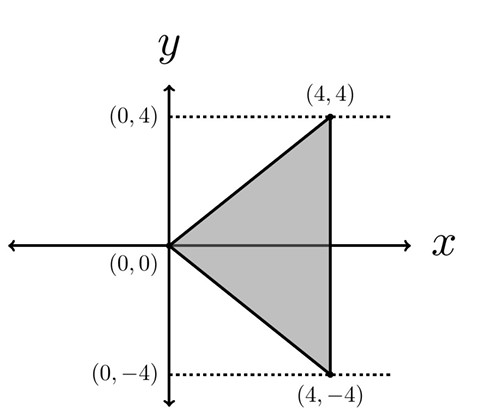
\includegraphics[width=0.5\columnwidth]{figs/m25.jpg}
        \caption*{}
        \label{fig:m25}
    \end{figure}
    
    \hfill{(GATE EC 2022)}

    \item A linear 2-port network is shown in Fig. \brak{a}.\figref{fig:m26}  An ideal DC voltage source of 10 V is connected across Port 1. A variable resistance R is connected across Port 2. As R is varied, the measured voltage and current at Port 2 is shown in Fig. \brak{b} as a $V_2$ versus $-I_2$ plot. Note that for $V_2 = 5$ V, $I_2 = 0$ mA, and for $V_2 = 4$ V, $I_2 = -4$ mA.
    When the variable resistance R at Port 2 is replaced by the load shown in Fig. \brak{c}, the current $I_2$ is \rule{2cm}{0.4pt} mA \brak{\text{rounded off to one decimal place}}.
    \begin{figure}[H]
        \centering
        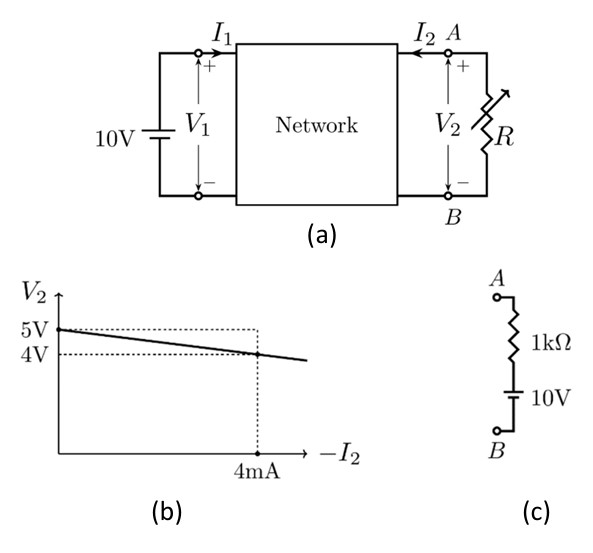
\includegraphics[width=\columnwidth]{figs/m26.jpg}
        \caption*{}
        \label{fig:m26}
    \end{figure}
    
    \hfill{(GATE EC 2022)}

    \item For a vector $\vec{x} = \sbrak{x\sbrak{0}, x\sbrak{1}, \dots, x\sbrak{7}}$, the 8-point discrete Fourier transform \brak{DFT} is denoted by $\vec{X} = \text{DFT}\brak{\vec{x}} = \sbrak{X\sbrak{0}, X\sbrak{1}, \dots, X\sbrak{7}}$, where
    \begin{align*}
    X\sbrak{k} = \sum_{n=0}^7 x\sbrak{n} \exp\brak{-j\frac{2\pi}{8}nk}.
    \end{align*}
    Here, $j = \sqrt{-1}$. If $\vec{x} = \sbrak{1, 0, 0, 0, 2, 0, 0, 0}$ and $\vec{y} = \text{DFT}\brak{\text{DFT}\brak{\vec{X}}}$, then the value of $y\sbrak{0}$ is \rule{2cm}{0.4pt} \brak{\text{rounded off to one decimal place}}.
    
    \hfill{(GATE EC 2022)}

    \item A p-type semiconductor with zero electric field is under illumination \brak{low level injection} in steady state condition. Excess minority carrier density is zero at $x = \pm 2l_n$, where $l_n = 10^{-4}$ cm is the diffusion length of electrons. Assume electronic charge, $q = -1.6 \times 10^{-19}$ C. The profiles of photo-generation rate of carriers and the recombination rate of excess minority carriers \brak{R} are shown.\figref{fig:m27}  Under these conditions, the magnitude of the current density due to the photo-generated electrons at $x = +2l_n$ is \rule{2cm}{0.4pt} mA/cm$^2$ \brak{\text{rounded off to two decimal places}}.
    \begin{figure}[H]
        \centering
        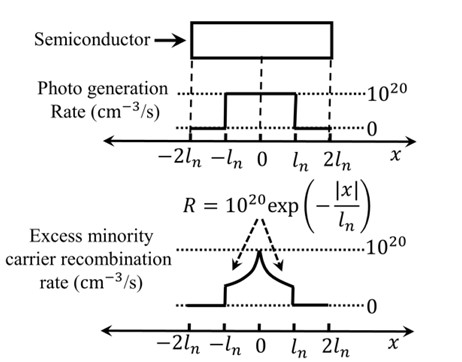
\includegraphics[width=\columnwidth]{figs/m27.jpg}
        \caption*{}
        \label{fig:m27}
    \end{figure}
    
    \hfill{(GATE EC 2022)}

    \item A circuit and the characteristics of the diode \brak{D} in it are shown.\figref{fig:m28}  The ratio of the minimum to the maximum small signal voltage gain $\frac{\partial V_{out}}{\partial V_{in}}$ is \rule{2cm}{0.4pt} \brak{\text{rounded off to two decimal places}}.
    \begin{figure}[H]
        \centering
        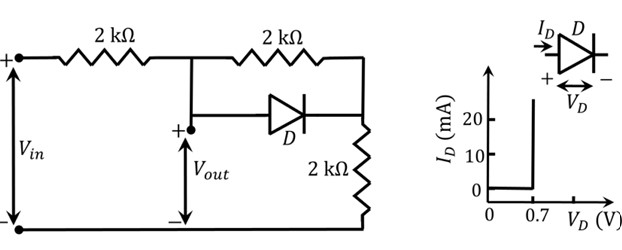
\includegraphics[width=\columnwidth]{figs/m28.jpg}
        \caption*{}
        \label{fig:m28}
    \end{figure}
    
    \hfill{(GATE EC 2022)}

    \item Consider the circuit shown\figref{fig:m29}  with an ideal OPAMP. The output voltage $V_o$ is \rule{2cm}{0.4pt} V \brak{\text{rounded off to two decimal places}}.
    \begin{figure}[H]
        \centering
        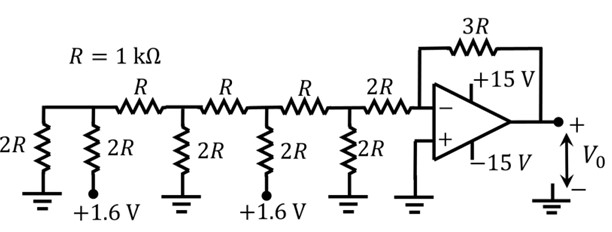
\includegraphics[width=0.5\columnwidth]{figs/m29.jpg}
        \caption*{}
        \label{fig:m29}
    \end{figure}
    
    \hfill{(GATE EC 2022)}

    \item Consider the circuit shown\figref{fig:m30}  with an ideal long channel nMOSFET \\ \brak{\text{enhancement-mode, substrate is connected to the source}}. The transistor is appropriately biased in the saturation region with $V_{GG}$ and $V_{DD}$ such that it acts as a linear amplifier. $v_i$ is the small-signal ac input voltage. $v_A$ and $v_B$ represent the small-signal voltages at the nodes A and B, respectively. The value of $\frac{v_A}{v_B}$ is \rule{2cm}{0.4pt} \brak{\text{rounded off to one decimal place}}.
    \begin{figure}[H]
        \centering
        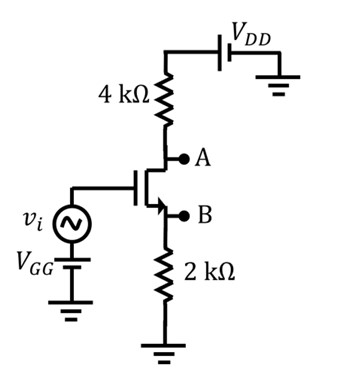
\includegraphics[width=0.4\columnwidth]{figs/m30.jpg}
        \caption*{}
        \label{fig:m30}
    \end{figure}
    
    \hfill{(GATE EC 2022)}

    \item The block diagram of a closed-loop control system is shown\figref{fig:m31}  in the figure. $R\brak{s}, Y\brak{s},$ and $D\brak{s}$ are the Laplace transforms of the time-domain signals $r\brak{t}, y\brak{t},$ and $d\brak{t},$ respectively. Let the error signal be defined as $e\brak{t} = r\brak{t} - y\brak{t}$. Assuming the reference input $r\brak{t} = 0$ for all $t$, the steady-state error $e\brak{\infty}$, due to a unit step disturbance $d\brak{t}$, is \rule{2cm}{0.4pt} \brak{\text{rounded off to two decimal places}}.
    \begin{figure}[H]
        \centering
        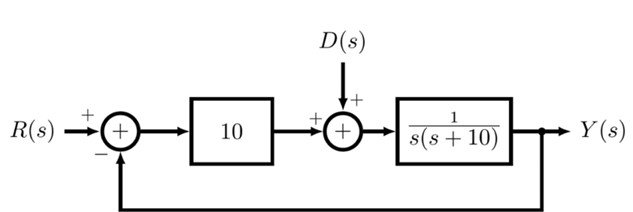
\includegraphics[width=0.3\columnwidth]{figs/m31.jpg}
        \caption*{}
        \label{fig:m31}
    \end{figure}
    
    \hfill{(GATE EC 2022)}

    \item The transition diagram of a discrete memoryless channel with three input symbols and three output symbols is shown in the figure.\figref{fig:m32}  The transition probabilities are as marked.
    The parameter $\alpha$ lies in the interval \sbrak{0.25, 1}. The value of $\alpha$ for which the capacity of this channel is maximized, is \rule{2cm}{0.4pt} \brak{\text{rounded off to two decimal places}}.
    \begin{figure}[H]
        \centering
        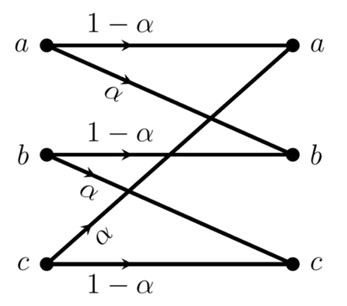
\includegraphics[width=0.3\columnwidth]{figs/m32.jpg}
        \caption*{}
        \label{fig:m32}
    \end{figure}
    
    \hfill{(GATE EC 2022)}

    \item Consider communication over a memoryless binary symmetric channel using a \brak{7, 4} Hamming code. Each transmitted bit is received correctly with probability $\brak{1-\epsilon}$, and flipped with probability $\epsilon$. For each codeword transmission, the receiver performs minimum Hamming distance decoding, and correctly decodes the message bits if and only if the channel introduces at most one bit error.
    For $\epsilon = 0.1$, the probability that a transmitted codeword is decoded correctly is \rule{2cm}{0.4pt} \brak{\text{rounded off to two decimal places}}.
    
    \hfill{(GATE EC 2022)}

    \item Consider a channel over which either symbol $x_A$ or symbol $x_B$ is transmitted. Let the output of the channel Y be the input to a maximum likelihood \brak{ML} detector at the receiver. The conditional probability density functions for Y given $x_A$ and $x_B$ are:
    \begin{align*}
        f_{Y|x_A}\brak{y} &= e^{-\brak{y+1}}u\brak{y+1}, \\
        f_{Y|x_B}\brak{y} &= e^{\brak{y-1}}\brak{1-u\brak{y-1}},
    \end{align*}
    where $u\brak{\cdot}$ is the standard unit step function. The probability of symbol error for this system is \rule{2cm}{0.4pt} \brak{\text{rounded off to two decimal places}}.
    
    \hfill{(GATE EC 2022)}
    
    \item Consider a real valued source whose samples are independent and identically distributed random variables with the probability density function, $f\brak{x}$, as shown in the figure.\figref{fig:m33} 
    \begin{figure}[H]
        \centering
        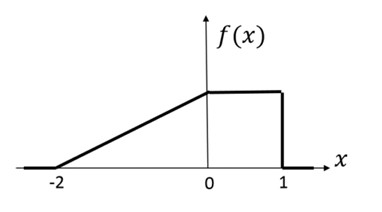
\includegraphics[width=0.4\columnwidth]{figs/m33.jpg}
        \caption*{}
        \label{fig:m33}
    \end{figure}
    Consider a 1 bit quantizer that maps positive samples to value $\alpha$ and others to value $\beta$. If $\alpha^*$ and $\beta^*$ are the respective choices for $\alpha$ and $\beta$ that minimize the mean square quantization error, then $\brak{\alpha^* - \beta^*} = $ \rule{2cm}{0.4pt} \brak{\text{rounded off to two decimal places}}.
    
    \hfill{(GATE EC 2022)}

    \item In an electrostatic field, the electric displacement density vector, $\vec{D}$, is given by
    \begin{align*}
     \vec{D}\brak{x, y, z} = \brak{x^3\vec{i} + y^3\vec{j} + xy^2\vec{k}} \text{ C/m}^2,
     \end{align*}
    where $\vec{i}, \vec{j}, \vec{k}$ are the unit vectors along x-axis, y-axis, and z-axis, respectively. Consider a cubical region R centered at the origin with each side of length 1 m, and vertices at \brak{\pm 0.5 m, \pm 0.5 m, \pm 0.5 m}. The electric charge enclosed within R is \rule{2cm}{0.4pt} C \brak{\text{rounded off to two decimal places}}.
    
    \hfill{(GATE EC 2022)}

\end{enumerate}

\end{document}